% Created 2025-06-14 sáb 21:15
% Intended LaTeX compiler: pdflatex
\documentclass[10pt]{article}
\usepackage[utf8]{inputenc}
\usepackage{lmodern}
\usepackage[T1]{fontenc}
\usepackage[top=1in, bottom=1.in, left=1in, right=1in]{geometry}
\usepackage{graphicx}
\usepackage{longtable}
\usepackage{float}
\usepackage{wrapfig}
\usepackage{rotating}
\usepackage[normalem]{ulem}
\usepackage{amsmath}
\usepackage{textcomp}
\usepackage{marvosym}
\usepackage{wasysym}
\usepackage{amssymb}
\usepackage{amsmath}
\usepackage[theorems, skins]{tcolorbox}
\usepackage[version=3]{mhchem}
\usepackage[numbers,super,sort&compress]{natbib}
\usepackage{natmove}
\usepackage{url}
\usepackage[cache=false]{minted}
\usepackage[strings]{underscore}
\usepackage[linktocpage,pdfstartview=FitH,colorlinks,
linkcolor=blue,anchorcolor=blue,
citecolor=blue,filecolor=blue,menucolor=blue,urlcolor=blue]{hyperref}
\usepackage{attachfile}
\usepackage{setspace}
\usepackage[spanish]{babel}
\usepackage{fontspec}
\date{}
\title{Tasa de fumadores vs tasa de incendios}
\begin{document}

\maketitle
\section*{Datos}
\label{sec:org9eb59b0}

Analizamos 20 observaciones anuales, recopiladas entre 2001 y 2021, correspondientes a:

\begin{description}
\item[{\texttt{Tasa\_Fumadores}}] Porcentaje de fumadores entre residentes adultos en USA (Fuente: CDC).
\item[{\texttt{Tasa\_Incendios}}] Número de incendios por cada 100.000 residentes en los USA (Fuente: FBI).
\end{description}

El objetivo es evaluar si existe soporte estadístico para la hipótesis de que la reducción progresiva en el porcentaje de fumadores incide directamente en la disminución del número de incendios. 

\begin{description}
\item[{Ficheros:}] Versión del ejercicio en \href{https://github.com/mbujosab/EconometriaAplicada-SRC/blob/main/FumadoresVsIncendios.pdf}{pdf}
\begin{itemize}
\item Datos: \url{FumadoresVsIncendios.gdt}
\item Guión de gretl: \url{FumadoresVsIncendios.inp}
\end{itemize}
\end{description}
\subsubsection*{Gráfico de las series y diagrama de dispersión}
\label{sec:org64872da}

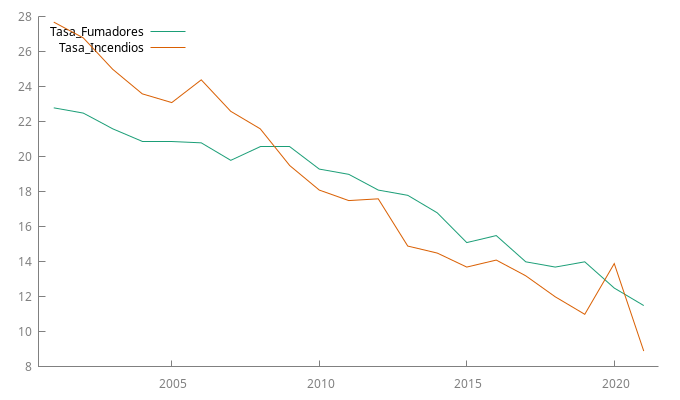
\includegraphics[width=0.5\textwidth]{./FumadoresVsIncendios/Tasa_FumadoresyTasa_Incendios.png} 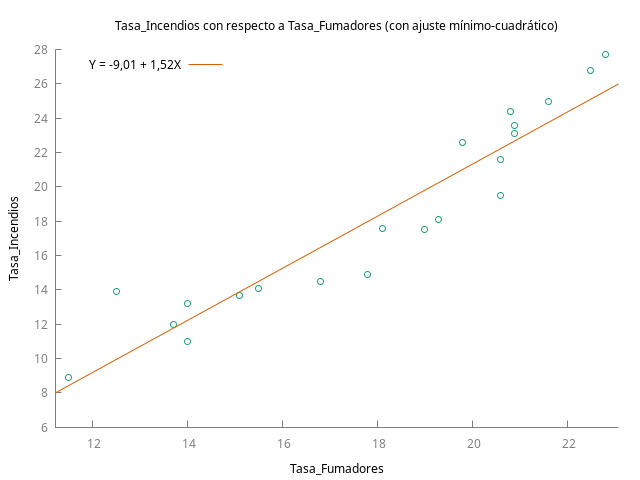
\includegraphics[width=0.5\textwidth]{./FumadoresVsIncendios/Tasa_IncendiosVsTasa_Fumadores.png}
\section*{Contrastes de raiz unitaria y de estacionariedad}
\label{sec:org3ac1b04}
\subsection*{\texttt{Tasa\_Fumadores}}
\label{sec:org7cb5c4c}
\subsubsection*{Contraste aumentado de Dickey Fuller para \texttt{Tasa\_Fumadores}}
\label{sec:orge655d85}

{\footnotesize
\begin{verbatim}
Contraste aumentado de Dickey-Fuller para Tasa_Fumadores
contrastar hacia abajo desde 4 retardos, con el criterio AIC
tamaño muestral 18
la hipótesis nula de raíz unitaria es: [a = 1]

  contraste con constante 
  incluyendo 2 retardos de (1-L)Tasa_Fumadores
  modelo: (1-L)y = b0 + (a-1)*y(-1) + ... + e
  valor estimado de (a - 1): 0,0822928
  estadístico de contraste: tau_c(1) = 1,41073
  valor p asintótico 0,9991
  Coef. de autocorrelación de primer orden de e: 0,049
  diferencias retardadas: F(2, 14) = 2,476 [0,1200]
\end{verbatim}
}
\subsubsection*{Conteste KPSS de estacionariedad para \texttt{Tasa\_Fumadores}}
\label{sec:orgc85c8a2}

{\footnotesize
\begin{verbatim}
Contraste KPSS para Tasa_Fumadores

T = 21
Parámetro de truncamiento de los retardos = 4
Estadístico de contraste = 0,534078

                      10%      5%      1%
Valores críticos: 0,357   0,462   0,697
Valor p interpolado 0,038
\end{verbatim}
}
\subsection*{\texttt{Tasa\_Incendios}}
\label{sec:org0446c40}

\subsubsection*{Contraste aumentado de Dickey Fuller para \texttt{Tasa\_Incendios}}
\label{sec:org47b8f8f}

{\footnotesize
\begin{verbatim}
Contraste aumentado de Dickey-Fuller para Tasa_Incendios
contrastar hacia abajo desde 4 retardos, con el criterio AIC
tamaño muestral 19
la hipótesis nula de raíz unitaria es: [a = 1]

  contraste con constante 
  incluyendo un retardo de (1-L)Tasa_Incendios
  modelo: (1-L)y = b0 + (a-1)*y(-1) + ... + e
  valor estimado de (a - 1): -0,0782544
  estadístico de contraste: tau_c(1) = -1,15001
  valor p asintótico 0,698
  Coef. de autocorrelación de primer orden de e: -0,097
\end{verbatim}
}
\subsubsection*{Conteste KPSS de estacionariedad para \texttt{Tasa\_Incendios}}
\label{sec:org38562b5}

{\footnotesize
\begin{verbatim}
Contraste KPSS para Tasa_Incendios

T = 21
Parámetro de truncamiento de los retardos = 4
Estadístico de contraste = 0,539254

                      10%      5%      1%
Valores críticos: 0,357   0,462   0,697
Valor p interpolado 0,037
\end{verbatim}
}
\section*{Regresión en niveles: \texttt{Tasa\_Incendios} sobre \texttt{Tasa\_Fumadores}}
\label{sec:org1a45e1f}

{\footnotesize
\begin{verbatim}
Modelo 2: MCO, usando las observaciones 2001-2021 (T = 21)
Variable dependiente: Tasa_Incendios

                  coeficiente  Desv. típica  Estadístico t  valor p 
  ------------------------------------------------------------------
  const            -9,01379      2,21156        -4,076      0,0006   ***
  Tasa_Fumadores    1,51665      0,120819       12,55       1,21e-10 ***

Media de la vble. dep.  18,27143   D.T. de la vble. dep.   5,555731
Suma de cuad. residuos  66,42434   D.T. de la regresión    1,869764
R-cuadrado              0,892399   R-cuadrado corregido    0,886736
F(1, 19)                157,5789   Valor p (de F)          1,21e-10
Log-verosimilitud      -41,88889   Criterio de Akaike      87,77778
Criterio de Schwarz     89,86683   Crit. de Hannan-Quinn   88,23116
rho                     0,455882   Durbin-Watson           1,019367


Contraste de la hipótesis nula de distribución Normal:
Chi-cuadrado(2) = 0,054 con valor p 0,97334


Contraste de heterocedasticidad de White

Estadístico de contraste: TR^2 = 0,140140,
con valor p = P(Chi-cuadrado(2) > 0,140140) = 0,932328


Contraste de Breusch-Godfrey para autocorrelación hasta el orden 4

Estadístico de contraste: LMF = 1,281174,
con valor p = P(F(4,15) > 1,28117) = 0,321

Estadístico alternativo: TR^2 = 5,347590,
con valor p = P(Chi-cuadrado(4) > 5,34759) = 0,253

Ljung-Box Q' = 9,19766,
con valor p = P(Chi-cuadrado(4) > 9,19766) = 0,0563
\end{verbatim}
}
\section*{Regresión en primeras diferencias: \texttt{d\_Tasa\_Incendios} sobre \texttt{d\_Tasa\_Fumadores}}
\label{sec:org229f929}

{\footnotesize
\begin{verbatim}
Modelo 4: MCO, usando las observaciones 2002-2021 (T = 20)
Variable dependiente: d_Tasa_Incendios

                    coeficiente  Desv. típica  Estadístico t  valor p
  -------------------------------------------------------------------
  const             -0,951343      0,467488      -2,035       0,0568  *
  d_Tasa_Fumadores  -0,0200761     0,531889      -0,03774     0,9703 

Media de la vble. dep. -0,940000   D.T. de la vble. dep.   1,558812
Suma de cuad. residuos  46,16435   D.T. de la regresión    1,601464
R-cuadrado              0,000079   R-cuadrado corregido   -0,055472
F(1, 18)                0,001425   Valor p (de F)          0,970307
Log-verosimilitud      -36,74353   Criterio de Akaike      77,48705
Criterio de Schwarz     79,47852   Crit. de Hannan-Quinn   77,87581
rho                    -0,614047   Durbin-Watson           2,429053


Contraste de la hipótesis nula de distribución Normal:
Chi-cuadrado(2) = 12,244 con valor p 0,00219


Contraste de heterocedasticidad de White

Estadístico de contraste: TR^2 = 1,380003,
con valor p = P(Chi-cuadrado(2) > 1,380003) = 0,501575


Contraste de Breusch-Godfrey para autocorrelación hasta el orden 4

Estadístico de contraste: LMF = 2,023163,
con valor p = P(F(4,14) > 2,02316) = 0,146

Estadístico alternativo: TR^2 = 7,326102,
con valor p = P(Chi-cuadrado(4) > 7,3261) = 0,12

Ljung-Box Q' = 4,62915,
con valor p = P(Chi-cuadrado(4) > 4,62915) = 0,328
\end{verbatim}
}

\newpage
\section*{Contrastes de raíz unitaria y de estacionariedad para los residuos \texttt{uhat} del modelo de regresión en niveles}
\label{sec:org2512beb}

\subsection*{Contraste aumentado de Dickey Fuller sobre la existencia de una raíz unitaria para \texttt{uhat}}
\label{sec:orgada8694}

{\footnotesize
\begin{verbatim}
Contraste aumentado de Dickey-Fuller para uhat
contrastar hacia abajo desde 4 retardos, con el criterio AIC
tamaño muestral 20
la hipótesis nula de raíz unitaria es: [a = 1]

  contraste con constante 
  incluyendo 0 retardos de (1-L)uhat
  modelo: (1-L)y = b0 + (a-1)*y(-1) + e
  valor estimado de (a - 1): -0,544803
  estadístico de contraste: tau_c(1) = -2,71633
  valor p asintótico 0,07119
  Coef. de autocorrelación de primer orden de e: -0,105
\end{verbatim}
}
\subsection*{Conteste KPSS de estacionariedad para \texttt{uhat}}
\label{sec:orgf38f934}

{\footnotesize
\begin{verbatim}
Contraste KPSS para uhat

T = 21
Parámetro de truncamiento de los retardos = 4
Estadístico de contraste = 0,165232

                      10%      5%      1%
Valores críticos: 0,357   0,462   0,697
Valor p > .10
\end{verbatim}
}
\section*{Preguntas}
\label{sec:org2953ca1}

\subsection*{Pregunta 1}
\label{sec:org1044afe}

(\textbf{1 pts.}) Utilice la información disponible en la sección \hyperref[sec:org9eb59b0]{Datos} y en la sección \hyperref[sec:org3ac1b04]{Contrastes de raiz unitaria y de estacionariedad} para discutir exhaustivamente si las series \texttt{Tasa\_Fumadores} y \texttt{Tasa\_Incendios} son realizaciones de procesos estacionarios en media o no.

(\hyperref[sec:org1d836a2]{Respuesta 1})
\subsection*{Pregunta 2}
\label{sec:org2a5c222}

(\textbf{1 pts.}) Discuta exhaustivamente la información que se muestra en la sección \hyperref[sec:org1a45e1f]{Regresión en niveles: \texttt{Tasa\_Incendios} sobre \texttt{Tasa\_Fumadores}}. Concretamente, comente 
\begin{enumerate}
\item la interpretación de los coeficientes de la regresión (constante y pendiente).
\item interpretación de los estadísticos de ajuste
\item evidencias sobre el cumplimiento o incumplimiento de los supuestos estándar del modelo de regresión lineal además de cualquier otro resultado que considere de interés.
\end{enumerate}

(\hyperref[sec:org1a04b04]{Respuesta 2})
\subsection*{Pregunta 3}
\label{sec:org8d61215}

(\textbf{1 pts.}) Compare de todas las formas posibles la \hyperref[sec:org1a45e1f]{regresión en niveles} con la \hyperref[sec:org229f929]{regresión en primeras diferencias} ¿Cuál de los dos modelos es más adecuado? ¿Qué se puede concluir sobre la relación entre ambas series?

(\hyperref[sec:orgbbeaf09]{Respuesta 3})
\subsection*{Pregunta 4}
\label{sec:orgb8b2484}

(\textbf{0.5 pts.}) Indique cuáles de las siguientes expresiones son correctas respecto del modelo correspondiente a la \hyperref[sec:org1a45e1f]{regresión en niveles} ajustada a los datos de \texttt{Tasa\_Incendios} (con un redondeo a tres decimales).
\begin{description}
\item[{Expresión 1}] \(\widehat{I_t} = -9.014 + 1.517\, (F_t)\)
\item[{Expresión 2}] \({I_t} = -9.014 + 1.517\, (F_t) +  \widehat{\varepsilon_t}\)
\item[{Expresión 3}] \({I_t} = -9.014 + 1.517\, (F_t)\)
\item[{Expresión 4}] \(\widehat{I_t} = -9.014 + 1.517\, (F_t) + \widehat{\varepsilon_t}\)
\end{description}
donde \(I_t\) denota la serie \texttt{Tasa\_Incendios}, \(F_t\) denota la serie \texttt{Tasa\_Fumadores} y \(\widehat{\varepsilon_t}\) es el residuo de la regresión correspondiente a la observación \emph{t}-ésima.

(\hyperref[sec:orgd2ab241]{Respuesta 4})
\subsection*{Pregunta 5}
\label{sec:org86b0685}

(\textbf{0.5 pts.}) Respecto al resultado del \hyperref[sec:org7cb5c4c]{test aumentado de Dickey-Fuller (ADF)} para \texttt{Tasa\_Fumadores}, discuta sobre la veracidad o falsedad de la siguiente afirmación:
\begin{quote}
\emph{No se rechaza la hipótesis nula de \textbf{estacionariedad} con un 5\% de significación}.
\end{quote}

(\hyperref[sec:orgfdf3e39]{Respuesta 5})
\subsection*{Pregunta 6}
\label{sec:orge014ae7}

(\textbf{0.5 pts.}) Respecto al resultado del \hyperref[sec:org7cb5c4c]{test KPSS} para \texttt{Tasa\_Fumadores}, discuta brevemente sobre la veracidad o falsedad de la siguiente afirmación:
\begin{quote}
\emph{Se rechaza la hipótesis nula de \textbf{estacionariedad} con un 5\% de significación}.
\end{quote}

(\hyperref[sec:orgf994f55]{Respuesta 6})
\subsection*{Pregunta 7}
\label{sec:orga095046}

(\textbf{0.5 pts.}) Respecto al resultado del \hyperref[sec:org0446c40]{test ADF} para \texttt{Tasa\_Incendios}, discuta brevemente sobre la veracidad o falsedad de la siguiente afirmación:
\begin{quote}
\emph{No se rechaza la hipótesis nula de \textbf{NO estacionariedad} con un 5\% de significación}.
\end{quote}

(\hyperref[sec:org1d2b1eb]{Respuesta 7})
\subsection*{Pregunta 8}
\label{sec:org4dca258}

(\textbf{0.5 pts.}) Respecto al resultado del \hyperref[sec:org0446c40]{test KPSS} para \texttt{Tasa\_Incendios}, discuta brevemente sobre la veracidad o falsedad de la siguiente afirmación:
\begin{quote}
\emph{Se rechaza la hipótesis nula de \textbf{NO estacionariedad} con un 5\% de significación}.
\end{quote}

(\hyperref[sec:org5ba66d1]{Respuesta 8})
\subsection*{Pregunta 9}
\label{sec:org5b2514e}

(\textbf{0.5 pts.}) En referencia al \hyperref[sec:org64872da]{\emph{``diagrama de dispersión''}} entre ambas tasas, discuta brevemente sobre la veracidad o falsedad de la siguiente afirmación:
\begin{quote}
\emph{Muestra que existe una relación causal entre las variables \texttt{Tasa\_Fumadores} y \texttt{Tasa\_Incendios}.}
\end{quote}

(\hyperref[sec:org66ff6be]{Respuesta 9})
\subsection*{Pregunta 10}
\label{sec:orge41fde9}

(\textbf{1 pts.}) Observe los contrastes de hipótesis que aparecen tras la \hyperref[sec:org1a45e1f]{regresión en niveles} y discuta brevemente sobre el cumplimiento de las hipótesis del modelo lineal general (MLG) en dicha regresión.

(\hyperref[sec:org0e46c64]{Respuesta 10})
\subsection*{Pregunta 11}
\label{sec:orgc7a6e69}

(\textbf{1 pts.}) Con un nivel de significación del 5\%, discuta si:
\begin{itemize}
\item los resultados que se muestran respecto a los \hyperref[sec:org3ac1b04]{Contrastes de raiz unitaria y de estacionariedad}
\item las regresiones en  \hyperref[sec:org1a45e1f]{niveles}
\item y los \hyperref[sec:org2512beb]{Contrastes de raíz unitaria y de estacionariedad para los residuos \texttt{uhat} del modelo de regresión en niveles}
\end{itemize}
sugieren conjuntamente que las series analizadas podrían estar \emph{cointegradas}.

(\hyperref[sec:org31c0c21]{Respuesta 11})
\subsection*{Pregunta 12}
\label{sec:orgb63c23f}

(\textbf{0.5 pts.}) Discuta brevemente sobre la veracidad o falsedad de la siguiente afirmación respecto a los \hyperref[sec:org2512beb]{Contrastes de raíz unitaria y de estacionariedad para los residuos \texttt{uhat} del modelo de regresión en niveles}:
\begin{quote}
\emph{Con un nivel de significación del 10\%, los resultados de los test ADF y KPSS son contradictorios}.
\end{quote}

(\hyperref[sec:org03606a8]{Respuesta 12})
\subsection*{Pregunta 13}
\label{sec:org138ff23}

(\textbf{0.5 pts.}) Discuta brevemente sobre la veracidad o falsedad de la siguiente afirmación:
\begin{quote}
\emph{La comparación de los resultados de la \hyperref[sec:org1a45e1f]{regresión en niveles} con la \hyperref[sec:org229f929]{regresión en primeras diferencias} sugiere que la relación entre \texttt{Tasa\_Incendios} y \texttt{Tasa\_Fumadores} podría ser espúria}.
\end{quote}

(\hyperref[sec:org178a5b6]{Respuesta 13})
\subsection*{Pregunta 14}
\label{sec:org663bf1c}

(\textbf{1 pts.}) Discuta brevemente sobre la veracidad o falsedad de la siguiente afirmación:
\begin{quote}
\emph{La estimación del término constante del modelo correspondiente a la \hyperref[sec:org229f929]{regresión en primeras diferencias} sugiere que, por cada año que pasa, cabe esperar que la incidencia de incendios se reduzca en aproximadamente \texttt{1} incendio menos por cada 100.000 residentes}.
\end{quote}

(\hyperref[sec:org6c82b00]{Respuesta 14})
\section*{Respuestas}
\label{sec:org2a45e96}

\subsection*{Respuesta 1}
\label{sec:org1d836a2}

\begin{itemize}
\item La primera figura muestra con claridad que ambas series temporales tienen una tendencia decreciente y que, por tanto, no podemos asumir que estas series sean realizaciones de procesos estocásticos estacionarios en media.

\item En cuanto a los resultados de la sección \hyperref[sec:org3ac1b04]{Contrastes de raiz unitaria y de estacionariedad}, los test ADF para las series \texttt{Tasa\_Fumadores} y \texttt{Tasa\_Incendios} no rechazan la hipótesis nula (\(H_0:\) la serie es integrada al menos de primer orden) para los niveles de significación habituales (10\%, 5\% 0 1\%), pues arrojan \emph{p}-valores de \texttt{0,991} y \texttt{0,698}, respectivamente.

\item Los resultados del test KPSS no son tan contundentes, ya que los \emph{p}-valores interpolados son de \texttt{0,038} para \texttt{Tasa\_Fumadores} y de \texttt{0,037} para \texttt{Tasa\_Incendios}. Por tanto, la hipótesis nula (\(H_0:\) la serie es estacionaria en media) se rechazaría al 5\% de significación, aunque no se rechazaría al 1\%.
\end{itemize}

En conjunto, podemos asumir que estos datos \textbf{no} son realizaciones de procesos estocásticos estacionarios (lo que coloquialmente se expresa diciendo que \emph{"estas series no son estacionarias en media"}).

(\hyperref[sec:org1044afe]{Pregunta 1})
\subsection*{Respuesta 2}
\label{sec:org1a04b04}

\begin{description}
\item[{Interpretación de los coeficientes de la regresión}] Ambos coeficientes estimados resultan ser estadísticamente significativos a los niveles de significación habituales (10\%, 5\% ó 1\%).

\begin{itemize}
\item El término constante NO admite una interpretación coherente. Intentar interpretarlo implicaría suponer que si \texttt{Tasa\_Fumadores} fuera 0 (\textbf{caso que no se observa en la muestra}) la tasa de incendios por cada 100.000 habitantes sería negativa. \emph{En este modelo la constante es un parámetro no interpretable}.

\item La pendiente indica que si la tasa de fumadores aumentase en un punto porcentual, el valor esperado estimado para la tasa de incendios crecería en 1,52 incendios por cada 100.000 residentes.
\end{itemize}

\item[{Interpretación de los indicadores de ajuste}] La desviación típica residual es de 1,87 incendios/100.000 residentes. Es una medida de la dispersión de los residuos.

El R-cuadrado es \texttt{0,89}. Como el \(R^2\) es un ratio entre la varianza muestral de los datos ajustados y la varianza muestral de los datos del regresando, el \(R^2\) se interpreta como una medida de la bondad del ajuste de los datos (el modelo ajustado capta el 89\% de la varianza muestral del regresando). 

El R-cuadrado corregido es un ratio de las correspondientes cuasivarianza que sirve para comparar el ajuste de distintos modelos anidados (i.e., modelos con el mismo regresando y donde los regresores de uno de los modelos son un subconjunto de los regresores del otro).

Los criterios de información de Akaike, Schwarz y Hannan Quinn toman los valores \texttt{87,78}, \texttt{89,87} y \texttt{88,23}, respectivamente. Se trata de otros medidas de ajuste que permiten comparar modelos con el mismo regresando, por lo que, sin otro modelo con el compararlos, no nos dan mucha información.

\item[{Evidencia sobre sobre el cumplimiento de los supuestos del modelo clásico de regresión lineal}] Los contrastes de normalidad, homoscedasticidad y ausencia de autocorrelación no rechazan a los niveles de significación habituales sus respectivas hipótesis nulas (\(H_0\): los datos provienen de una distribución normal; \(H_0\): los datos son realizaciones de variables aleatorias con la misma varianza; y \(H_0\): los datos provienen de variables aleatorias que no muestran correlación serial).
\end{description}

(\hyperref[sec:org2a5c222]{Pregunta 2})
\subsection*{Respuesta 3}
\label{sec:orgbbeaf09}

Al comparar modelos, lo habitual es fijarse tanto en estadísticos de ajuste, como en el cumplimiento de las hipótesis del MLG y la consistencia de los resultados.

\begin{description}
\item[{Estadísticos de ajuste}] En este caso, en el que estos modelos ajustan variables distintas (\texttt{Tasa\_Incendios} en el primer caso y \texttt{d\_Tasa\_Incendios} en el segundo), por tanto \textbf{los estadísticos de ajuste no son comparables}.

No obstante, es evidente que la primera regresión muestra un elevado \(R^2\) (el ajuste reproduce un elevado porcentaje de la varianza muestral de la \texttt{Tasa\_Incendios}) y que, sin embargo, la segunda regresión muestra un bajísimo \(R^2\) (un paupérrimo ajuste de los datos). Aunque no cabe comparar los R-cuadrado corregidos ya que estos modelos no están anidados (como se apuntaba más arriba).

\item[{Cumplimiento de hipótesis}] Todos los parámetros del modelo de la primera regresión son significativos. Los test residuales no rechazan las hipótesis nulas de normalidad, homoscedasticidad y ausencia de autocorrelación.

El ajuste del segundo modelo tiene un parámetro no significativo y sus residuos rechazan la hipótesis nula de normalidad.

\item[{Consistencia de los resultados de la primera regresión en niveles}] Si la relación entre las variables fuera como la que implica la primera regresión (que aparentemente es la muestra un buen ajuste de los datos y no evidencia incumplimientos del los supuestos clásicos), es decir, si realmente  $$\boldsymbol{y}=\beta_1\boldsymbol{1}+\beta_2\boldsymbol{x}+\boldsymbol{u}.$$ Entonces también debería ser cierto que $$\nabla\boldsymbol{y}=\beta_2\nabla\boldsymbol{x}+\nabla\boldsymbol{u}.$$
\end{description}

Sin embargo, en la \hyperref[sec:org229f929]{Regresión en primeras diferencias: \texttt{d\_Tasa\_Incendios} sobre \texttt{d\_Tasa\_Fumadores}} la única variable estadísticamente significtiva la constante (que debería ser cero). 
Es decir, la \hyperref[sec:org229f929]{Regresión en primeras diferencias: \texttt{d\_Tasa\_Incendios} sobre \texttt{d\_Tasa\_Fumadores}} \textbf{contradice la posibilidad de que ambas variables estén relacionadas}. Es decir, los resultados de la primera regresión no son consistentes con los de la segunda. Dicho de otro modo, los resultados de la segunda estimación indican que estamos ante un caso de correlación espúria, ya que la relación entre ambas variables se vuelve no significativa al diferenciarlas.

A este respecto, podemos argumentar que, pese a los estadísticos de significación y los de ajuste, el segundo modelo es mejor que el primero; ya que refleja que ambas variables no están relacionadas, es decir, que fumar menos no afecta significativamente en la incidencia de incendios.

(\hyperref[sec:org8d61215]{Pregunta 3})
\subsection*{Respuesta 4}
\label{sec:orgd2ab241}

Dado que  \(\widehat{\varepsilon_t}\) es el residuo de la regresión correspondiente a la observación \emph{t}-ésima; es decir, que \(\widehat{\varepsilon_t}={I_t}-\widehat{I_t}\), sólo las dos primeras expresiones son correctas. La primera corresponde a los valores ajustados \(\widehat{I_t}\) y, por tanto, la segunda expresión resulta ser \({I_t}=\widehat{I_t}+\widehat{\varepsilon_t}\): es decir, la regresión descompone los datos observados en \emph{datos ajustados} más el \emph{error cometido por dicho ajuste}.

(\hyperref[sec:orgb8b2484]{Pregunta 4})
\subsection*{Respuesta 5}
\label{sec:orgfdf3e39}

La afirmación es FALSA. La hipótesis nula del test es \(H_0:\) \emph{la serie es NO estacionaria}.

(\hyperref[sec:org86b0685]{Pregunta 5})
\subsection*{Respuesta 6}
\label{sec:orgf994f55}

La afirmación es VERDADERA. La hipótesis nula del test KPSS es \(H_0:\) \emph{la serie es estacionaria}; y el p valor interpolado (3,8\%) da lugar a un rechazo al 5\% de significación.

(\hyperref[sec:orge014ae7]{Pregunta 6})
\subsection*{Respuesta 7}
\label{sec:org1d2b1eb}

La afirmación es VERDADERA. La hipótesis nula del test es \(H_0:\) \emph{la serie es NO estacionaria} y el p valor (69,8\%) da lugar a un no rechazo al 5\% de significación.

(\hyperref[sec:orga095046]{Pregunta 7})
\subsection*{Respuesta 8}
\label{sec:org5ba66d1}

La afirmación es FALSA. La hipótesis nula del test es \(H_0:\) \emph{la serie es estacionaria}.

(\hyperref[sec:org4dca258]{Pregunta 8})
\subsection*{Respuesta 9}
\label{sec:org66ff6be}

La afirmación es FALSA. Dos variables pueden estar fuertemente correladas sin que exista una relación causal entre ellas. Esto sucede, por ejemplo, si la correlación entre ambas es espúria.

(\hyperref[sec:org5b2514e]{Pregunta 9})
\subsection*{Respuesta 10}
\label{sec:org0e46c64}

En primer lugar, independientemente de los resultados que arrojen los test, los contrastes de hipótesis no pueden dar una garantía plena sobre el cumplimiento de las hipótesis. Además, no se incluyen contrastes para todas las hipótesis; por ejemplo, no se muestra un test de linealidad.

Pese a todo ello, los test mostrados NO inducen a rechazar las
correspondientes hipótesis nulas a los niveles de significación habituales (\(H_0\): distribución normal, \(H_0\): homocedasticidad y \(H_0\): ausencia de autocorrelación).

(\hyperref[sec:orge41fde9]{Pregunta 10})
\subsection*{Respuesta 11}
\label{sec:org31c0c21}

A un 5\% de significación 
\begin{itemize}
\item a) los \hyperref[sec:org3ac1b04]{Contrastes de raiz unitaria y de estacionariedad} realizados sugieren que ambas series son no estacionarias.
\item b) la \hyperref[sec:org1a45e1f]{regresion en niveles} indica que existe una relación significativa entre ambas variables, y
\item c) por otra parte, los \hyperref[sec:org2512beb]{Contrastes de raíz unitaria y de estacionariedad para los residuos \texttt{uhat} del modelo de regresión en niveles} no se refuerzan, ya que el ADF no rechaza su hipótesis nula (\textbf{no estacionariedad}) por un margen pequeño (7,1\% frente a 5\%) y el KPSS tampoco rechaza la suya (\textbf{estacionariedad}).
\end{itemize}

Consecuentemente, a la luz de estos resultados, las series podrían estar cointegradas, aunque la conclusión de la etapa 4 es dudosa, ya que según el ADF no habría cointegración al 5\%, mientras que el KPSS no la descarta.

(\hyperref[sec:orgc7a6e69]{Pregunta 11})
\subsection*{Respuesta 12}
\label{sec:org03606a8}

La afirmación es FALSA. A un 10\% de significación el test ADF rechaza la hipótesis nula (\textbf{no estacionariedad}) y el KPSS no rechaza su hipótesis nula (\textbf{estacionariedad}). Por tanto, ambos contraste no se contradicen a este nivel de significación.

(\hyperref[sec:orgb63c23f]{Pregunta 12})
\subsection*{Respuesta 13}
\label{sec:org178a5b6}

Efectivamente la afirmación es VERDADERA. La regresión en niveles es muy significativa. En primeras diferencias no hay relación. Por tanto, la apariencia de relación se debe, sencillamente, a que ambas series son realizaciones de procesos no estacionarios.

(\hyperref[sec:org138ff23]{Pregunta 13})
\subsection*{Respuesta 14}
\label{sec:org6c82b00}

La afirmación es VERDADERA. El valor estimado del término constante (\texttt{-0,951}) está muy próximo a \texttt{-1} y puede interpretarse como el valor esperado del cambio en \texttt{Tasa\_Incendios}, en ausencia de efectos de la variable explicativa (que en cualquier caso no afecta significativamente a la endógena).

(\hyperref[sec:org663bf1c]{Pregunta 14})
\end{document}
